\documentclass[a4paper]{article}

\usepackage[english]{babel}
\usepackage[utf8]{inputenc}
\usepackage{amsmath}
\usepackage{graphicx}
\usepackage[colorinlistoftodos]{todonotes}

\usepackage{theorem}
\usepackage{amssymb}
\usepackage{bm}
\usepackage{booktabs}
\usepackage[colorlinks=TRUE,linkcolor=olive,citecolor=brown]{hyperref}

\usepackage{caption}
\usepackage{subcaption}
\usepackage{natbib}

\newenvironment{proof}{{\bf Proof:  }}{\hfill\rule{2mm}{2mm}}

\newtheorem{fact}{Fact}[section]
\newtheorem{lemma}[fact]{Lemma}
\newtheorem{theorem}[fact]{Theorem}
\newtheorem{definition}[fact]{Definition}
\newtheorem{corollary}[fact]{Corollary}
\newtheorem{proposition}[fact]{Proposition}
\newtheorem{claim}[fact]{Claim}
\newtheorem{exercise}[fact]{Exercise}
\newtheorem{remark}[fact]{Remark}

\usepackage{algorithm}
\usepackage{algorithmic}

\makeatletter
\newcommand{\distas}[1]{\mathbin{\overset{#1}{\kern\z@\sim}}}%
\newsavebox{\mybox}\newsavebox{\mysim}
\newcommand{\distras}[1]{%
  \savebox{\mybox}{\hbox{\kern3pt$\scriptstyle#1$\kern3pt}}%
  \savebox{\mysim}{\hbox{$\sim$}}%
  \mathbin{\overset{#1}{\kern\z@\resizebox{\wd\mybox}{\ht\mysim}{$\sim$}}}%
}
\makeatother

\newcommand{\RT}[1]{\marginpar{\footnotesize\color{red}RT: #1}}

\newcommand{\Ex}{\mathbb{E}}

\bibliographystyle{plainnat}

\title{Law of Large Graphs}

\date{\today}

\begin{document}
\maketitle

\begin{abstract}
Estimating the mean of a population of graphs based on a sample is a core problem in network science.
While using the element-wise sample mean of the adjacency matrices is a common approach, this method does not exploit any underlying structure of graphs.
We propose using a low-rank method together with tools for dimension selection and diagonal augmentation to improve performance over the naive methodology.
Theoretical results for the stochastic blockmodel show that this method will offer major improvements when there are many vertices.
Similarly, in analyzing human connectome data, we demonstrate that the low-rank methods outperform the the standard sample mean.
These results indicate that low-rank methods should be a key part of the tool box for researchers studying populations of graphs.
\end{abstract}

\section{Introduction}

Estimation of the mean of a population based on a sample is at the core of statistics.
The sample mean, motivated by the law of large numbers and the central limit theorem, has its place as one of the most important statistics for this task.
Nowadays we take averages almost everywhere, from data in Euclidean space to more complex objects, like shapes, documents and graphs.

The mean of a population of graphs is a high dimensional object, consisting of $O(N^2)$ parameters for a graph with $N$ vertices.
Estimating high dimensional estimands with a small sample size using naive unbiased methods often leads to inaccurate estimates with very high variance.
By exploiting the bias-variance trade-off, it is often fruitful to develop estimators which have some bias with greatly reduced variance.
When these estimators are biased towards low-dimensional structures which well approximate the full dimensional population mean, major improvements can be realized.


Additionally, in a striking result, \citet{stein1956inadmissibility} and \citet{james1961estimation} showed the arithmetic average should not always be the first choice and is inadmissable in even simple settings by todays standards. 
Twenty-seven years later, \citet{gutmann1982stein} proved that this phenomenon cannot occur when the sample spaces are finite.
But even when  the sample mean is admissible, it doesn't close the door to other estimators in all cases.
In many situations where other structural information is hypothesized, for instance a collection of graphs as considered in this paper, other estimators may be preferable.

In complex data settings such as shape data, language data or graph data, we also must take care in how we define the mean.
As with real valued data, one may want to define the mean of a graph to itself be a graph such as for the median graph \citep{jiang2001median}.
However, this may be too restrictive for populations of graphs where there is high variation in which edges appear. 
Instead, we define the mean graph as the weigted adjacency matrix with weights given by the proportion of times the corresponding edge appears in the population. 
This population mean is becoming more and more important both in statistical inference and in various applications like connectomics, social networks, and computational biology.

% Nowadays, people care about information that can be extracted from the networks through different ways in neuroscience.
\citet{ginestet2014hypothesis} proposed a way to test if there is a difference between the distributions for two groups of networks.  
While hypothesis testing is the end goal of their work, estimation is a key intermediate step which may be improved by accounting for underlying structure in the mean matrix. 
Thus improving the estimation procedures for the mean graph is not only important by itself, but also can be applied to help improve other statistical inference procedures.

The element-wise sample mean is a reasonable estimator if we consider the general independent edge model (IEM) \cite{bollobas2007phase} without taking any additional structure into account. 
However, it does not perform very well especially when only a small sample size is available.
Intuitively, an estimator incorporating the mean-graph structure is preferable to the entry-wise MLE. 
In general, we don't have any knowledge about this structure so it can be hard to take advantage of in practice.



One of the most important structures in graphs is the community structure in which vertices are clustered into groups that share similar connectivity structure. The stochastic blockmodel (SBM) \cite{holland1983stochastic} is one model that captures this structural property and is widely used in modeling networks.
More generally, the latent positions model (LPM) \cite{hoff2002latent}, provides a way to parameterize the graph structure by latent positions associated with each vertex. 
Latent position models can capture strong community structure like the stochastic blockmodel, but may also allow for more variance within communities and other structures.
One example of a LPM which captures this middle ground is the random dot product graph (RDPG) \cite{young2007random, nickel2007random} which motivates our estimator. 
% In this paper, we analyze our estimator in terms of RDPG specifically.

Using the estimates of the latent positions based on a truncated eigen-decomposition of the adjacency matrix,  in the RDPG setting we consider an estimator for the mean of the collection of graphs which captures the low-rank structure of the RDPG model.
These estimates will improve performance since they will be biased towards the low-rank structure of the RDPG model and will have significantly lower overall variance than naive element-wise sample means.
In this study, we show via theory, simulations and real data analysis that it frequently outperforms the element-wise MLE, especially in small sample sizes.


% (Future work) Robust estimation, dimension selection, diagonal augmentation, etc.



\section{Models and Estimators}
\label{section:model_estimator}
This work considers the scenario of having $M$ graphs represented as adjacency matrices, $\{A^{(m)}\}$ ($m = 1, \cdots, M$), each having $N$ vertices.
We assume there is a known correspondence for vertices in different graphs, so that vertex $i$ in graph $m$ corresponds to vertex $i$ in graph $m'$ for any $i$, $m$, $m'$.
The graphs we consider are undirected and unweighted with no self-loops, so each $A^{(m)}$ is a binary symmetric matrix with zeros along the diagonal. An example application of this arises in the field of connectomics, where functional brain imaging data for each subject can be represented as a graph.
Each vertex represent a well defined anatomical region present in each subject, and an edge between two regions is defined to exist if correlation in activity between the regions surpasses a certain threshold.
Similarly, for structural brain imaging an edge may represent the presence of anatomical connections between the two regions.

For the purpose of this paper, we will also assume that the graphs are sampled independently and identically from some distribution.
We consider three nested models for these distributions, the independent edge model, the random dot product model, and the stochastic blockmodel, and two estimators motivated by these models.



\subsection{Independent Edge Model}
The first model we consider is the independent edge model (IEM) with parameter $P \in [0,1]^{N\times N}$ \citep{bollobas2007phase}.
An edge exists between vertex $i$ and vertex $j$ with probability $P_{ij}$ and each edge is present independently of all other edges. 
For this case, the mean graph is the 
For this case, we aim to estimate the mean matrix $P=\Ex[A^{(m)}]$ base on the observed adjacency matrices $A^{(1)},\dotsc,A^{(M)}$.



\subsection{Estimator $\bar{A}$}
Under the IEM, the MLE for the mean graph $P$ is the element-wise sample mean of the adjacency matrices $\bar{A}=\frac{1}{M}\sum_{m=1}^M A^{(m)}$.
It is unbiased with entry-wise variance $\mathrm{Var}(\bar{A}_{ij}) = P_{ij} (1-P_{ij})/M$. Moreover, $\bar{A}$ is the uniformly minimum-variance unbiased estimator, so it has the smallest variance among all unbiased estimators and enjoys the many asymptotic properties of the MLE as $M\to \infty$.

However, $\bar{A}$ doesn't exploit any graph structure, and sometimes the performance is not very good especially when $M$ is small. 
For example, when $M=1$, $\bar{A}$ is exactly the binary graph we observe, which is an inaccurate estimate for an arbitrary $P$ compared to estimates which exploit underlying structure.
Additionally, there are no useful asymptotic properties for $\bar{A}$ as the number of vertices $N$ becomes large.



\subsection{Random Dot Product Graph}
In graphs, the adjacencies between vertices generally depend on unobserved properties of the corresponding vertices. For example, in a connectomics setting, the two brain regions with similar properties will have similar connectivity patterns to other regions of the brain.
The latent positions graph (LPG) model proposed by Hoff et. al. (2002) \cite{hoff2002latent} captures such structure, where each vertex is associated with a latent position that influences the adjacencies for that vertex.
In this model, each vertex $i$ has an associated latent vector $X_i \in \mathbb{R}^d$.
Based on the latent positions, the existence of edges are conditionally independent with probability that only depends on the latent vectors of the incident vertices through a link function. If $d$ is much smaller than the number of vertices $N$ and the link function is known, LPMs are more parsimonious models compared to IEM, requiring only $dN$ parameters rather then $\binom{N}{2}$.

A specific instance of a LPM that we examine in this work is the random dot product graph model (RDPG) \cite{young2007random, nickel2007random} where the link function is the dot product, so the probability of an edge being present between two nodes is the dot product of their latent vectors.

Formally, let $\mathcal{X} \subset \mathbb{R}^d$ be a set such that $x, y \in \mathcal{X}$ implies $\left \langle  x,y \right \rangle =\sum_i x_i y_i \in [0, 1]$.
Let $X_1,\dotsc,X_n\in \mathcal{X}$ and write $X = [X_1|\cdots|X_N]^T \in \mathbb{R}^{N \times d}$.
A random graph $G$ with adjacency matrix $A$ is said to be an RDPG if
\[
    \Pr[A|X] = \prod_{i<j} \left \langle X_i, X_j \right \rangle^{A_{ij}} \left( 1 - \left \langle X_i, X_j \right \rangle \right)^{1 - A_{ij}}.
\]
In the RDPG model, each vertex $i$ is associated with latent position $X_i$ and  conditioned on the latent positions $X$, the edges $A_{ij} \distas{iid} \text{Bern}(\left \langle X_i, X_j \right \rangle)$.
Note that the probability matrix is the outter product of the latent position matrix with itself, $P = X X^T$.
This imposes two properties on $P$, namely that $P$ is positive-semidefinite and $\mathrm{rank}(P)=\mathrm{rank}(X)\leq d$.
These properties lead us to our proposed estimator.
%Note that $\mathrm{rank}(P) = \mathrm{rank}(X)$.




\subsection{Low-Rank Estimator $\hat{P}$}

Motivated by the low-rank structure of the RDPG mean matrix, we consider the estimator $\hat{P}$ based on the spectral decomposition of $\bar{A}$ which yields a low rank approximation of $\bar{A}$.
This estimator is similar to the estimator proposed by \citet{chatterjee2015matrix} but we analyze its performance more specifically in the random graph setting.

For a given dimension $d$ we consider the estimator $\hat{P}$ defined as the best rank-$d$ positive-semidefinite approximation of $\bar{A}$.
Since the graphs are symmetric, we can compute the eigendecomposition of $\bar{A}$ as $\hat{U} \hat{S} \hat{U}^T + \tilde{U}\tilde{S}\tilde{U}^T$, where $\hat{S}$ is a diagonal matrix with non-increasing entries along the diagonal corresponding to the largest $d$ eigenvalues of $A$ and $\hat{U}$ has columns given by the corresponding eigenvectors.
The $d$-dimensional adjacency spectral embedding (ASE) of $\bar{A}$ is given by $\hat{X}=\hat{U} \hat{S}^{1/2}\in \mathbb{R}^{N \times d}$.
For an RDPG, the rows of $\hat{X}$ are estimates of the latent vectors for each vertex \citep{sussman2014consistent}.
Using the adjacency spectral embedding, we have that $\hat{P} = \hat{X} \hat{X}^T=\hat{U}\hat{S}\hat{U}^T$.

To compute $\hat{P}$, we need to specify what rank $d$ to use and there are various ways of dealing with dimension selection. 
In this paper, we use Zhu and Ghodsi's elbow selection method \cite{zhu2006automatic} and the universal singular value thresholding (USVT) method \cite{chatterjee2015matrix}. 
Details are discussed in Section \ref{section:dim_select}.

Moreover, since the adjacency matrices are hollow, with zeros along the diagonal, there is a missing data problem that leads to inaccuracies if we compute $\hat{P}$ based only on $\bar{A}$. 
To compensate for this issue, we use an iterative method developed by Scheinerman and Tucker \cite{scheinerman2010modeling}. 
Details are discussed in Section \ref{section:diag_aug}.


\begin{algorithm}[H]
\caption{Algorithm to compute $\hat{P}$}
\label{algo:basic}
\begin{algorithmic}[1]
\STATE \textbf{Input:} $A^{(1)}, A^{(2)}, \cdots, A^{(M)}$, each $A^{(m)} \in \{0,1\}^{N \times N}$, $k_max$
\STATE Calculate the sample mean $\bar{A} = \frac{1}{M}\sum\limits_{m = 1}^M A^{(m)}$;
\STATE Calculate the scaled degree matrix $D^{(0)} = \mathrm{diag}(\bar{A} \bm{1})/(n-1)$;
\STATE Select the dimension $d$  using $\bar{A} + D^{(0)}$ (see Section \ref{section:dim_select});
\STATE Calculate the rank-$d$ approximation $\hat{U} \hat{S} \hat{U}^T$ for $\bar{A} + D^{(0)}$;
\STATE Update the diagonal to $D^{(1)} \leftarrow \mathrm{diag}(\hat{U} \hat{S} \hat{U}^T)$ (see Section \ref{section:diag_aug}); 
\STATE Set $\tilde{P}\rightarrow\hat{U} \hat{S} \hat{U}^T$, the rank-$d$ approximation for $\bar{A} + D^{(1)}$;
\STATE \textbf{Output}: $\hat{P}$ equal to $\tilde{P}$ with values $<0$ set to $0$ and values $>1$ set to $1$.
\end{algorithmic}
\end{algorithm}


Algorithm~\ref{algo:basic} gives the steps involved to compute the low-rank estimate $\hat{P}$.
As we will see in the proceeding sections, this procedure will frequently yield improvements in estimation as compared to using the sample mean $\bar{A}$.
While this is unsurprising for random dot product graphs, where we are able to show theoretical results to this effect, we also see this effect for connectome data and more general independent edge graphs.
In the next sections, we explore this estimator in the context of the stochastic blockmodel.

\subsection{Stochastic Block Model as an Random Dot Product Graph}
\label{section:sbm_rdpg}
One of the most important structures for graphs is the community structure in which vertices are clustered into different communities such that vertices of the same community behave similarly. This structural property is captured by the stochastic blockmodel (SBM) \cite{holland1983stochastic}, where each vertex is assigned to a block and the probability that an edge exists between two vertices depends only on their respective block memberships.

The SBM is parameterized by the number of blocks $K$ (generally much less than the number of vertices $N$), the block probability matrix $B \in [0,1]^{K \times K}$, and the vector of block memberships
 % and block proportion vector $\rho \in (0,1)^K$ with $\sum_{k=1}^K \rho_k = 1$. 
$\tau\in\{1,\dotsc,K\}^n$, where for each $i \in [n]$, $\tau_i = k$ means vertex $i$ is a member of block $k$.
% We will assume each vertex is assigned its block independently according to the probability vector $\rho$, so $\Pr[tau_i = k] = \rho_k$. 
Conditioned on $\tau$, each entry of the adjacency matrix $A_{ij}$ is independently sampled from the Bernoulli distribution with parameter $B_{\tau_i,\tau_j}$.

In order to analyze the estimator $\hat{P}$ motivated by RDPG, we move to another representation of SBM based on RDPG. 
Consider a positive semi-definite $K$-block SBM with a rank $d\le K$ block probability matrix $B$, we can always decompose $B$ into $\nu \nu^T$, where $\nu \in \mathbb{R}^{K \times d}$ and each row $\nu_k$ is the shared latent position for all vertices assigned to block $k$. 
For $X \in \mathbb{R}^{N \times d}$ with rows given by $X_i = \nu_{\tau_i}$, we have
\[
    \Pr[A_{ij} = 1|\tau] = B_{\tau_i, \tau_j} = \nu_{\tau_i}^T \nu_{\tau_j}.
\]
In this way, the SBM can be seen as an RDPG where all vertices in the same block will have identical latent positions.

An example SBM is illustrated in Fig~\ref{fig:SBM_example}.
We consider a 5-block SBM and plot the corresponding probability matrix and one adjacency matrix generated from it with 200 vertices. From the figure, we can clearly see the structure of 25 blocks in both the probability matrix and the adjacency matrix as a result of 5 different blocks among vertices.

\begin{figure}
\centering
\begin{subfigure}{.5\textwidth}
  \centering
  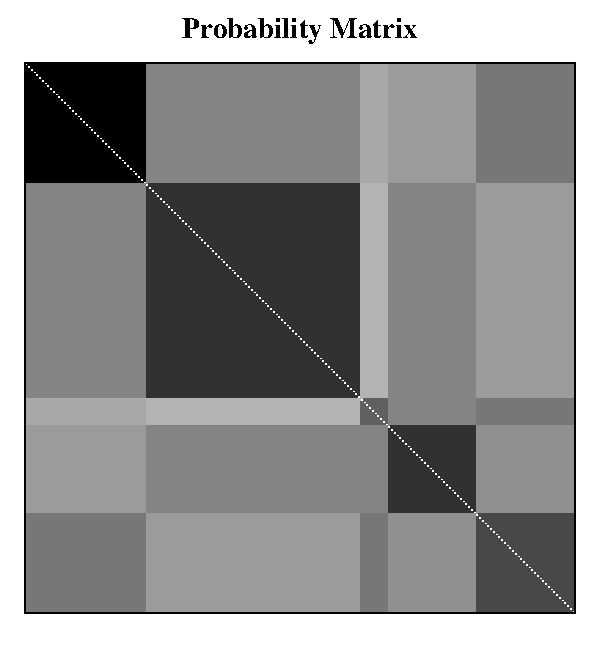
\includegraphics[width=\linewidth]{SBM_P.pdf}
\end{subfigure}%
\begin{subfigure}{.5\textwidth}
  \centering
  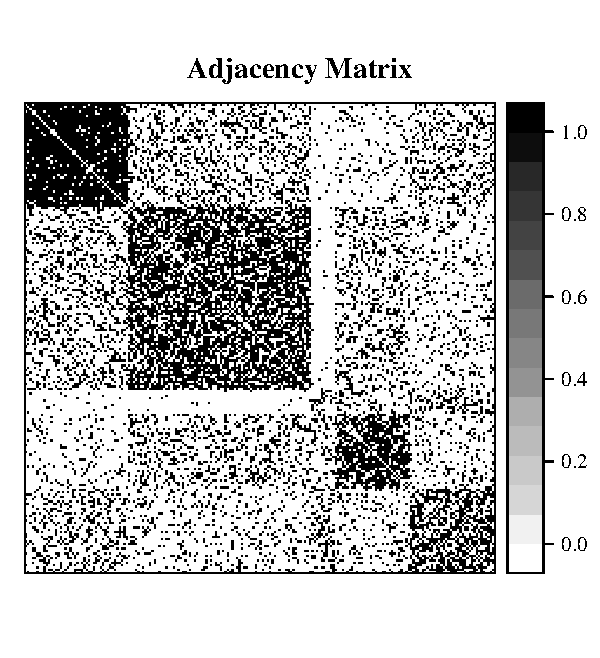
\includegraphics[width=\linewidth]{SBM_A.pdf}
\end{subfigure}
\caption{Example illustrating the stochastic blockmodel. The left figure shows the mean graph $P$ with $K = 5$ blocks and $N=200$ vertices and the right figure shows an adjacency matrix $A$ sampled according to the probabilities from $P$.
While $A$ is a noisy version of $P$, much of the structure of $P$ is preserved in $A$, a property we will exploit in our estimation procedure.
}
\label{fig:SBM_example}
\end{figure}



\section{Results}

\subsection{Theoretical Results}
\label{section:theoretical_result}
To estimate the mean of a collection of graphs, we consider the two estimators from Section \ref{section:model_estimator}: the entry-wise sample mean $\bar{A}$ and the low-rank $\hat{P}$ motivated by the RDPG.
In this section, we analyze the performance of these two estimators under the SBM by computing the entry-wise relative efficiency (RE), defined as $\mathrm{RE}(\bar{A}_{ij}, \hat{P}_{ij}) = \frac{\mathrm{MSE}(\hat{P}_{ij})}{\mathrm{MSE}(\bar{A}_{ij})}$.
Specifically, we consider the asymptotic relative efficiency as the number of vertices $N\to\infty$ but with the number of graphs $M$ fixed.

For this asymptotic framework, we assume where the block memberships $\tau_i$ are drawn iid from a multinomial distribution with block membership probabilities given by $\rho\in[0,1]^K$.
We will also assume that for a given $N$, the block membership probability are fixed for all graphs.
Denote block probability matrix $B = \nu \nu^T$. 
By definition, the mean of the collection of graphs generated from this SBM is $P$, where $P_{ij} = B_{\tau_i, \tau_j}$. After observing $M$ graphs on $N$ vertices $A^{(1)}, \cdots, A^{(M)}$ sampled independently from the SBM conditioned on $\tau$, we can calculate the two estimators $\bar{A}$ and $\hat{P}$.

\begin{lemma}
\label{lm:VarPhat}
For the above setting, for any $i, j$, if $\mathrm{rank}(B)=K=d$, we have
\[
    \lim_{N \to \infty} N \cdot \mathrm{Var}(\hat{P}_{ij}) =
    \frac{1/\rho_{\tau_i} + 1/\rho_{\tau_j}}{M} P_{ij} (1 - P_{ij}),
\]
and for large enough $N$, we have
\[
    \Ex[(\hat{P}_{ij} - P_{ij})^2] \approx
    \frac{1/\rho_{\tau_i} + 1/\rho_{\tau_j}}{M N} P_{ij}(1-P_{ij}).
\]
\end{lemma}

The proof of this lemma is outlined in Section \ref{section:outline_proof} and is based on results for the variance of the adjacency spectral embedding from \citet{athreya2013limit}. From the result, we can see that the MSE of $\hat{P}_{ij}$ is of order $O(M^{-1}N^{-1})$ approximately.

Moreover, since $\bar{A}_{ij}$ is the sample mean of $M$ independent Bernoulli random variables with parameter $P_{ij}$, we have
\[
    \Ex[(\bar{A}_{ij} - P_{ij})^2] = \frac{P_{ij}(1-P_{ij})}{M}.
\]
This yields the following result.
\begin{theorem}
\label{thm:ARE}
In the same setting as in Lemma \ref{lm:VarPhat}, for any $i$ and $j$, if $\mathrm{rank}(B)=K=d$, the asymptotic relative efficiency (ARE) is 
\[
    \mathrm{ARE}(\bar{A}_{ij}, \hat{P}_{ij}) = \lim_{N \to \infty} \mathrm{RE}(\bar{A}_{ij}, \hat{P}_{ij}) = 0.
\]
and for large enough $N$, we have
\[
    \mathrm{RE}(\bar{A}_{ij}, \hat{P}_{ij}) \approx
    \frac{1/\rho_{\tau_i} + 1/\rho_{\tau_j}}{N}.
\]
\end{theorem}

This theorem indicates that under the SBM, $\hat{P}$ is a much better estimate of the mean of the collection of graphs $P$ than $\bar{A}$. 
From the result, we see that the relative efficiency is of order $O(N^{-1})$ and $N \cdot \mathrm{RE}(\bar{A}_{ij}, \hat{P}_{ij})$ converges to $1/\rho_{\tau_i}+1/\rho_{\tau_j}$ when $N$ goes to infinity.
If for example there is one block containing half the vertices, the relative efficiency for estimating the probabilities of edges between vertices in that block will be approximately $4/N$.
For even large blocks the relative will decrease towards $1/N$ where as if a block tends to have very few vertices, so that the the asymptotic relative efficiency will tends towards 1, but will always be less than one.
Also, the ARE does not depend on the number of graphs $M$, so the larger the graphs are, the better $\hat{P}$ is relative to $\bar{A}$, regardless of $M$.

If instead of assuming that the graphs follow a SBM distribution we assume the graphs are distributed according to a RDPG distribution, similar gains in relative efficiency can be realized.
While there is no compact analytical formula for the relative efficiency of $\hat{P}$ versus $\bar{A}$ in the general RDPG case, using the same ideas as in Theorem~\ref{thm:ARE}, we can show that $\mathrm{RE}(\bar{A}_{ij},\hat{P}_{ij}) = O(1/N)$.

\begin{remark}
As we noted above, if the graphs are distributed according to an SBM or an RDPG, the relative efficiency is approximately invariant to the number of graphs $M$ when $N$ is large.
If on the other hand, the graphs are generated according to a full-rank independent edge model, then the relative efficiency can change more dramatically as $M$ changes. 
The reason for this is because for larger $M$, more of the eigenvectors of $\bar{A}$ will begin to concentrate around the eigenvectors of the mean graph.
This leads to the fact that the optimal embedding dimension will increase, making $\bar{A}$ and and the low-rank approximation at the optimal dimension closer together. 
As a result, $\mathrm{RE}(\bar{A},\hat{P})$ will increase as $M$ increases for full-rank models.
\end{remark}

\subsection{Validation with Simulations}\label{sec:sbm_sim}


\begin{figure}[!htb]
    \centering
    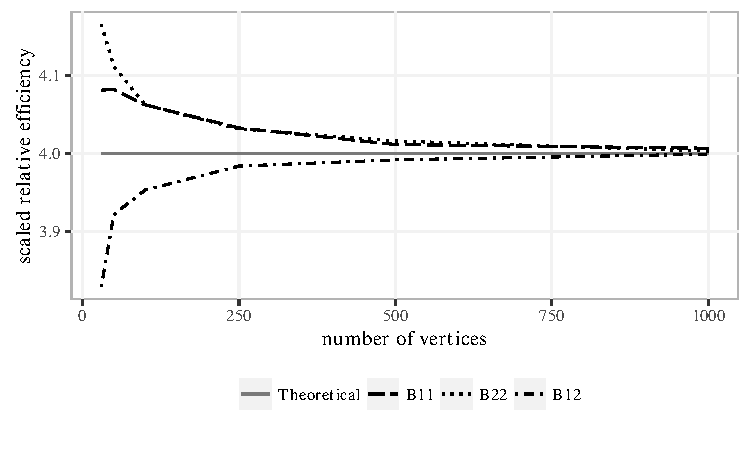
\includegraphics[width=1\textwidth]{RE.pdf}
    \caption{Scaled relative efficiency $N\cdot RE(\bar{A},\hat{P})$ as a function $N$ for fixed $M$ based on 1000 Monte Carlo replicates of the SBM from Section~\ref{sec:sbm_sim}.
    Each line represents the estimated scaled relative efficiency for one of the three distinct probabilities from the stochastic blockmodel.
    All the lines converge to four, the theoretical limit, as $N\to\infty$ since there are two blocks of equal size so $1/\rho_s+1/\rho_t=4$. }
    % Different types of dashed lines denote the simulated scaled RE associated with different blocks. Solid line represents the theoretical value for scaled RE. Observe that $N \cdot \mathrm{RE}_{st}(\bar{A}, \hat{P})$ converges to $1/\rho_s + 1/\rho_t = 4$ as expected.}
    \label{fig:RE}
\end{figure}

\begin{figure}[!t]
\centering
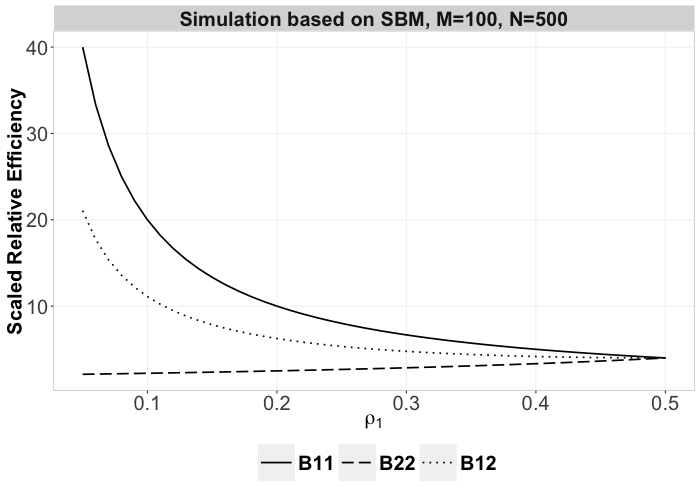
\includegraphics[width=1\textwidth]{Rho.pdf}
\caption{Theoretical scaled relative efficiency $N\cdot RE(\bar{A},\hat{P})$ for the three distinct edge probabilities as a function the proportion $\rho_1$ of vertices in the first block based on the SBM described in Section~\ref{sec:sbm_sim}.
These lines all meet at a scaled relative efficiency of 4 when $\rho_1=1/2$.
Improvements using low-rank methods are greater for larger blocks, such as for $B_{22}$ when $\rho_2=1-\rho_1$ is close to 1, while the improvements are smaller for blocks with relatively few vertex pairs such as $B_{11}$ and $B_{12}$ when $\rho_1$ is small.
% Simulated results for scaled RE, i.e. $N \cdot \mathrm{RE}_{st}(\bar{A}, \hat{P})$ with $N = 500$ and $M = 100$ of 1000 Monte Carlo replicates while changing $\rho_1$ from 0.1 to 0.9. Scaled relative efficiency in average with different $N$ and fixed $M$ based on 1000 Monte Carlo replicates. Different types of lines denote the simulated values associated with the edges we are averaging over. Notice that when $\rho_1 = 0.5$, the scaled RE has value $4.0$, which agrees with the result in Fig~\ref{fig:RE} as expected.}
}
\label{fig:RErho}
\end{figure}

In this section, we will illustrate the theoretical results from Section 3.1 regarding the relative efficiency between $\bar{A}$ and $\hat{P}$ via Monte Carlo simulation experiments.

%\subsubsection{Simulation Setting}
Here, we consider a 2-block SBM with parameters
\begin{equation*}
B = \begin{bmatrix}
0.42 & 0.2 \\
0.2 & 0.7
\end{bmatrix}
,\qquad \rho = \begin{bmatrix}
0.5 & 0.5
\end{bmatrix}.
\end{equation*}
When calculating $\hat{P}$, we omit the dimension selection step from Algorithm~\ref{algo:basic} and instead using the true dimension $d = \mathrm{rank}(B) = 2$.

%\subsubsection{Simulation Results}
To investigate the finite sample relative efficiency, we first sample 1000 Monte Carlo replicates from the above SBM distribution with different number of vertices $N$ and fixed number of graphs $M$. The scaled relative efficiency $N \cdot \mathrm{RE}(\bar{A}_{ij}, \hat{P}_{ij})$ can be estimated since $P$ is known for this simulation. Since the relative efficiency only depends on the blocks memberships of the pair $i,j$, we estimate the relative efficiency for each block pair using
\[
    \mathrm{RE}_{st}(\bar{A},\hat{P}) = \frac{\sum_{\tau_i=s,\tau_j=t,i \ne j} \widehat{MSE}(\hat{P}_{ij})}{\sum_{\tau_i=s,\tau_j=t,i \ne j} \widehat{MSE}(\bar{A}_{ij})}
\]
for $s,t\in\{1,2\}$, where $\hat{MSE}$ denotes the estimated mean square error based on the Monte Carlo replicates.

We plot the scaled relative efficiency $N \cdot \mathrm{RE}_{st}(\bar{A},\hat{P})$ in Fig~\ref{fig:RE}. 
Based on the Theorem~\ref{thm:ARE}, we have that the scaled RE converges to $1/\rho_{\tau_i}+1/\rho_{\tau_j}=4$ as $N\to\infty$ for all $i,j$.
This is plotted as a solid line.
The different dashed lines denote the estimated scaled RE associated with different block pairs, either $B_{11}$, $B_{12}$ or $B_{22}$. 
From the figure, we see that $N \cdot \mathrm{RE}_{st}(\bar{A}, \hat{P})$ converges to scaled asymptotic RE quite rapidly.
We omit error bars as the standard errors are very small for these estimates.
% {\color{red} Say something about why $B_{11}, B_{22}>4$ and $B_{12}<4$}



To further illustrate Theorem \ref{thm:ARE}, Fig~\ref{fig:RErho} shows $1/\rho_s + 1/\rho_t$, the scaled asymptotic RE, as $\rho$ changes from $0.01$ to $0.50$, for fixed $N=500$ and $M=100$.
For $N=500$ and $M=100$, estimates of the scaled RE based on simulations agree very closely with their corresponding theoretical values. Note that when $\rho_1 = 0.5$, the scaled RE has value $4.0$, which agrees with the result in Fig~\ref{fig:RE}.



\subsection{CoRR Brain Graphs: Cross-Validation}\label{sec:corr_data}

In practice, graphs do not follow the independent edge model, let alone an RDPG or SBM, but the mean of a collection of graphs is still of interest for these cases.
To demonstrate that the estimator $\hat{P}$ is still useful in such cases, we test its performance on structural connectomic data. 
The graphs are based on diffusion tensor MR images collected and available at the Consortium for Reliability and Reproducibility (CoRR) \citep{zuo2014open, gorgolewski2015high}.

The dataset contains 454 different brain scans, each of which was processed to yield an undirected, unweighted graph with no self-loops, using the pipeline describe in \citet{gray2013migraine} and \citet{kiar2016m2g}.
The vertices of the graphs represent different regions in the brain defined according to an atlas.
We used three atlases, the JHU atlas with 48 vertices, the Desikan atlas with 70 vertices and the  CPAC200 atlas with 200.
An edge exists between two vertices whenever there is at least one white-matter tract connecting the corresponding two regions of the brain. 
Further details of the dataset are provided in Section \ref{section:data}.

In order to evaluate the performance of the two estimators, we use a cross validation on the 454 graphs of each size. 
Specifically, for a given atlas, each Monte Carlo replicate corresponds to sampling $M$ graphs out of the 454 and computing the low-rank estimator $\hat{P}$ and the sample mean $\bar{A}$ using the $M$ selected graphs. 
We then compare these estimates to the sample mean for the remaining $454-M$ adjacency matrices.
While we cannot interpret this mean graph as the probability matrix for an IEM distribution (see section~\ref{sec:sim_iem}, it matches our definition as the proportion of times each edge appears in the population.

% By observing 454 graphs generated by the atlas being picked, we use $\hat{P}$ to estimate the mean graph $P$, which is the proportions of the existence of a white-matter tract connecting different parts of the brain. Since $P$ is unknown in practice, we perform a cross-validation study to compare $\bar{A}$ and $\hat{P}$. For each Monte Carlo replicate, we first fix the sample size $M$ and randomly sample $M$ graphs from the total 454 graphs in the dataset. We assure $M$ to be relatively small such that the entry-wise mean of the remaining $(454 - M)$ graphs is a valid approximation of the true probability matrix $P$ we are estimating. Then we can calculate $\bar{A}$ and $\hat{P}$ based on the $M$ samples and compare their performance based on the estimated probability matrix.

We run 1000 simulations on each of the three atlases for each sample size $M=1,5,10$.
We also considered all possible dimensions for $\hat{P}$ by ranging $d$ from 1 to $N$ in order to investigate the impact of the dimension selection procedures.
We plot the MSE of $\bar{A}$ and $\hat{P}$ in Fig~\ref{fig:realdata}.
The horizontal axis gives dimension $d$, which only impacs $\hat{P}$, which is why the MSE of $\bar{A}$ is shown as flat.

When $d$ is small, $\hat{P}$ underestimate the dimension and throws away important information, which leads to relatively poor performance. When $d=N$, $\hat{P}$ is equal to $\bar{A}$, so that the curve of the MSE for $\hat{P}$ ends at the MSE for $\bar{A}$. 
In practice, we use algorithms like Zhu and Ghodsi's method or USVT to select the dimension $d$ (see section~\ref{section:dim_select}). 
In the figure, we denote the 3rd elbow found by the Zhu and Ghodsi method by a triangle , and denote the dimension selected by USVT with threshold 0.7 by a square. 
% (with largest 95\% confidence interval length to be $3.5$)
% (with largest 95\% confidence interval length to be $0.7$)
Both dimension selection algorithms tend to select dimensions which nearly minimize the mean square error.
% The standard error for the Zhu and Ghodsi and the USVT methods are about $0.9$ and $0.17$ respectively.

When $M$ is 1 or 5, $\bar{A}$ has large variance which leads to large MSE. Meanwhile, $\hat{P}$ reduces the variance by taking advantages of inherent low-rank structure of the mean graph. Additionally, we see that there is a large range of dimensions where the performance for $\hat{P}$ is superior to $\bar{A}$. 
With a larger $M$, the performance of $\bar{A}$ improves so that its performance is frequently superior to $\hat{P}$ but $\hat{P}$ still performs nearly as well.

As further evidence for the improvement using $\hat{P}$, even when the dimension must be derived from data, Table~\ref{tab:corr_re} shows relative efficiencies of $\hat{P}$ versus $\bar{A}$.
For each atlas and each sample size we compare the \citet{zhu2006automatic} with the USVT method and note that both perform well relative to the full-dimensional $\bar{A}$, especially for large $N$ and small $M$.

\begin{figure}[!htb]
\centering
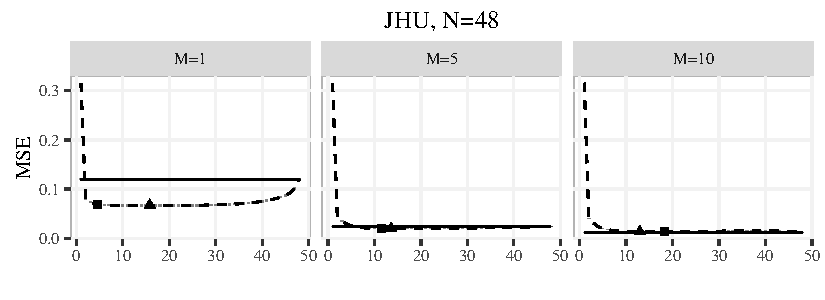
\includegraphics[width=1\textwidth]{corr_data_MSE_jhu.pdf}\\
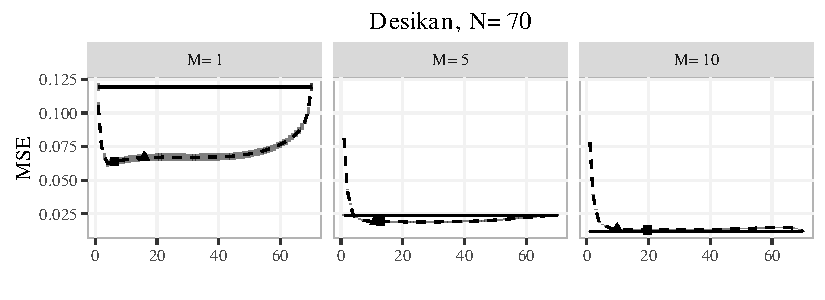
\includegraphics[width=1\textwidth]{corr_data_MSE_desikan.pdf}\\
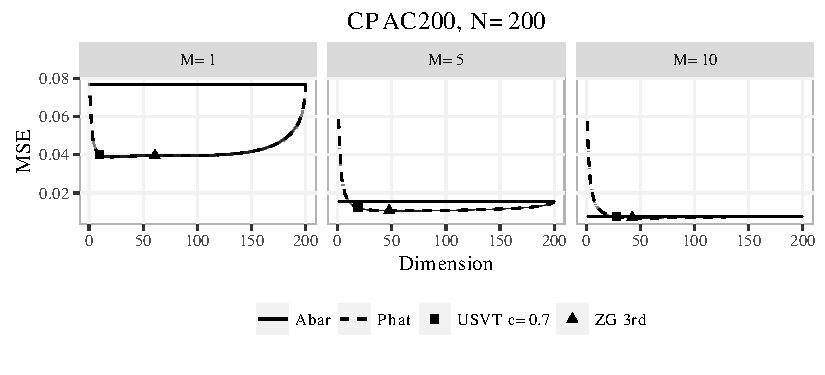
\includegraphics[width=1\textwidth]{corr_data_MSE_CPAC200.pdf}
\caption{A comparison of the mean square error for $\bar{A}$ (solid line) and $\hat{P}$ (dashed line) for three dataset (JHU, Desikan and CPAC200) while embedding the graphs into different dimensions and with different sample sizes $M$. The average dimensions chosen by the 3rd elbow of Zhu and Ghodsi is denoted by a triangle
 % (with largest 95\% confidence interval length to be $3.5$), 
 and chosen by USVT with threshold equals 0.7 is denoted in square.
% (with largest 95\% confidence interval length to be $0.7$). 
 Vertical intervals, visible mainly in the $N=48,70$ and $M=1$ plots, represent the 95\% confidence interval for the mean square errors.  When $M$ is small, $\hat{P}$ outperforms $\bar{A}$ with a flexible range of the embedding dimension including the average of the dimensions selected by Zhu and Ghodsi and USVT.}
\label{fig:realdata}
\end{figure}

\begin{table}[!htb]
    \caption{Relative efficiencies for estimating the mean graph for each atlas for the CoRR data set. We compared different sample sizes $m$ and different dimension selection procedures, ZG and USVT. Overall, the relative efficiencies are greater for smaller sample sizes $m$ and larger number of vertices $N$. } 
    \label{tab:corr_re}
    \centering

\begin{tabular}{rccc}\toprule
        % & $m=1$  & $m=5$  & $m=10$ \\\toprule
\multicolumn{1}{l}{\textbf{JHU}} & $m=1$  & $m=5$  & $m=10$  \\\midrule
ZG      & 0.54 & 0.81 & 1.14 \\
USVT    & 0.56 & 0.84 & 1.12 \\\midrule
\multicolumn{1}{l}{\textbf{Desikan}} & $m=1$  & $m=5$  & $m=10$  \\ \midrule
ZG      & 0.52 & 0.81 & 1.14 \\
USVT    & 0.50 & 0.81 & 1.09 \\\midrule
\multicolumn{1}{l}{\textbf{CPAC200}} & $m=1$  & $m=5$  & $m=10$  \\\midrule
ZG      & 0.51 & 0.68 & 0.89 \\
USVT    & 0.52 & 0.79 & 0.99 \\\bottomrule
\end{tabular}
\end{table}



As an illustration, we consider a random sample of size $M=5$ based on the Desikan atlas.
We calculated $\bar{A}$ and $\hat{P}$, using  Zhu and Ghodsi's 3rd elbow to select $d=11$. 
In Fig~\ref{fig:Matrix_desikan_m5}, the estimates $\bar{A}$ and $\hat{P}$ as well as the sample mean of 454 graphs (as a close estimate of $P$) are plotted. 
Since the sample size is small, there are a lot of pairs of vertices with no edges or 5 edges in the 5 observations.
This leads to the white and black pixels in the image corresponding to $\bar{A}$.
On the other hand, $\hat{P}$ has a finer gradient of values which in this case leads to a more accurate estimate.

Moreover, Fig~\ref{fig:Diff_desikan_m5} shows the values for the absolute estimation error $|\bar{A} - P|$ and $|\hat{P}-P|$. The lower triangular sections shows the actual absolute difference while the upper triangular matrix highlights the vertex pairs with absolute differences larger than 0.4. 
There are 18 edges from $\bar{A}$ and 6 edges from $\hat{P}$ being highlighted in the figure, further indicating the superior performance of $\hat{P}$.
Note that $\approx 13\%$ of the potential edges are present in all $454$ graphs and hence $\bar{A}$ will always have zero error for those pairs of vertices.
Nonetheless, $\hat{P}$ typically outperforms $\bar{A}$.

To investigate the difference in performance with respect to the geometry of brain, 
in Fig~\ref{fig:Diff_between_desikan}, we plot the 50 edges with the largest difference $|\bar{A} - P| - |\hat{P} - P|$ according to the location of the corresponding regions in the brain. Red edges indicate that $\hat{P}$ overestimate $P$ while blue means that $\hat{P}$ underestimate $P$. The edge width is determined by the estimation error for $\hat{P}$, where pairs with larger estimation error are represented by thicker lines.
We also highlight the regions corresponding to vertices that contribute most to the difference, meaning the vertices $i$ with the largest value of $\sum_j (|\bar{A} - P| - |\hat{P} - P|)_{ij}$.
Notably, these regions of improvement appear to be concentrated in three distinct regions of the brain. 
The top five regions are the inferior temporal, middle temporal, and transverse temporal regions in the left hemisphere and the parahippocampal and parsopercularis regions in the right hemisphere of the Desikan atlas.

These results demonstrate that $\hat{P}$ gives a better estimate than $\bar{A}$ for the CoRR dataset with all three atlases. 
Importantly, this improvement is robust to the embedding dimension as long as provided the dimension is not underestimated.

\begin{figure}[!htb]
\centering
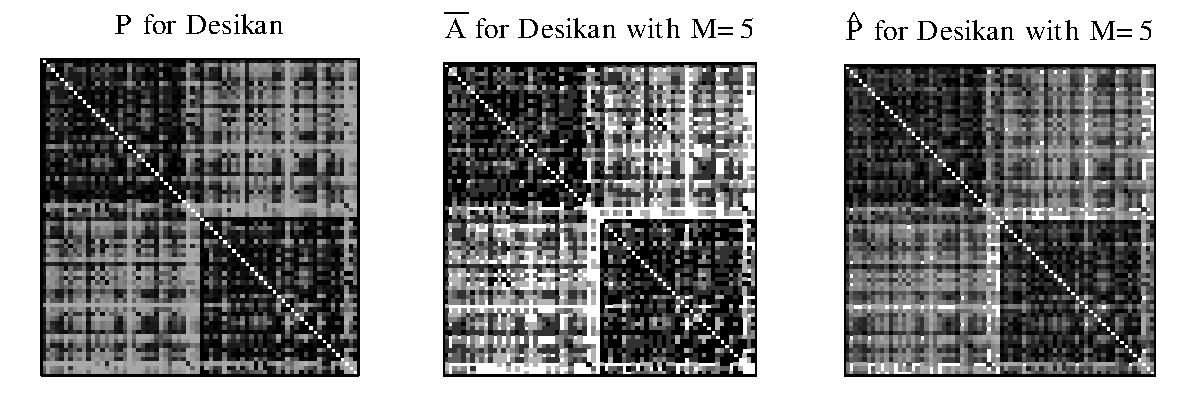
\includegraphics[width=1\textwidth]{Matrix_desikan_m5.pdf}
\caption{Heat maps indicatign the sample mean for the remaining $454-5$ graphs (left), sample mean for the 5 sampled graphs (center), and $\hat{P}$ for the 5 sampled graphs with dimension $d=11$ selected using the Zhu and Ghodsi method (right).
Darker pixels indicated a higher probability of an edge between the given vertices.
Note that $\hat{P}$ appears to be better estimate the true probabilities $P$, especially for edges between the two hemispheres, in the upper right (and lower left) block.
}
\label{fig:Matrix_desikan_m5}
\end{figure}

\begin{figure}

\begin{center}
  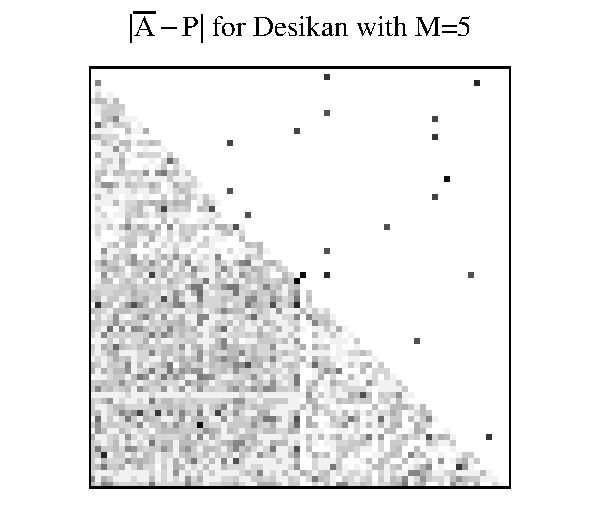
\includegraphics[height=.4\linewidth]{Diff2_desikan_m5.pdf}\hspace{-12pt}
  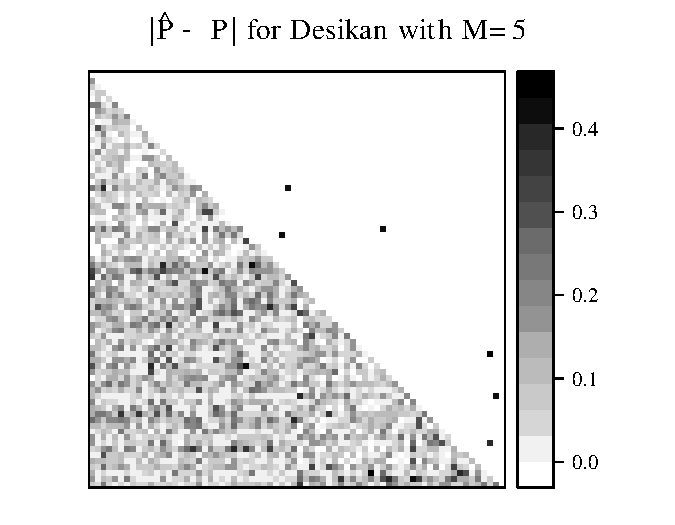
\includegraphics[height=.4\linewidth]{Diff3_desikan_m5.pdf}
\end{center}

\caption{Heat plot of the absolute estimation error $|\bar{A} - P|$ and $|\hat{P} - P|$ for a sample of size $M=5$ from Desikan dataset while embedding the graphs into dimension $d=11$ selected by the 3rd elbow of ZG method. The lower triangular matrix shows the actual absolute difference, while the upper triangular matrix only highlights the edges with absolute differences larger than $0.4$. The fact that 18 edges from $\bar{A}$ are highlighted and while only six edges from $\hat{P}$ are highlighted indicates that $\hat{P}$ suffers from fewer large outliers.}
\label{fig:Diff_desikan_m5}
\end{figure}

\begin{figure}[!htb]
\centering
\includegraphics[width=1\textwidth]{Diff_between_desikan.png}
\caption{Top 5 regions of the brain (vertices in graphs) and top 50 connections between regions (edges in graphs) with largest difference $|\bar{A} - P| - |\hat{P} - P|$. Red edges indicate that $\hat{P}$ overestimate $P$ while blue means that $\hat{P}$ underestimate $P$. The edge width is determined by the estimation error. Connections with larger estimation error are represented by thicker lines. This figure shows the regions and connections of the brain where $\hat{P}$ outperforms $\bar{A}$ the most for estimating $P$.}
\label{fig:Diff_between_desikan}
\end{figure}


%\begin{figure}[!htb]
%\centering
%\includegraphics[width=1\textwidth]{JHU.png}
%\caption{Comparison of MSE between $\bar{A}$ (solid line) and $\hat{P}$ (dashed line) for JHU dataset while embedding the graphs into different dimensions with different size $M$ of the subsamples. The dimension chosen by the 3rd elbow of Zhu and Ghodsi is denoted in triangle, and chosen by USVT with threshold equals 0.7 is denoted in square. Vertical intervals represent the 95\% confidence interval. When $M$ is small, $\hat{P}$ outperforms $\bar{A}$ with a flexible range of the embedding dimension including what Zhu and Ghodsi selects.}
%\label{fig:JHU}
%\end{figure}
%
%\begin{figure}[!htb]
%\centering
%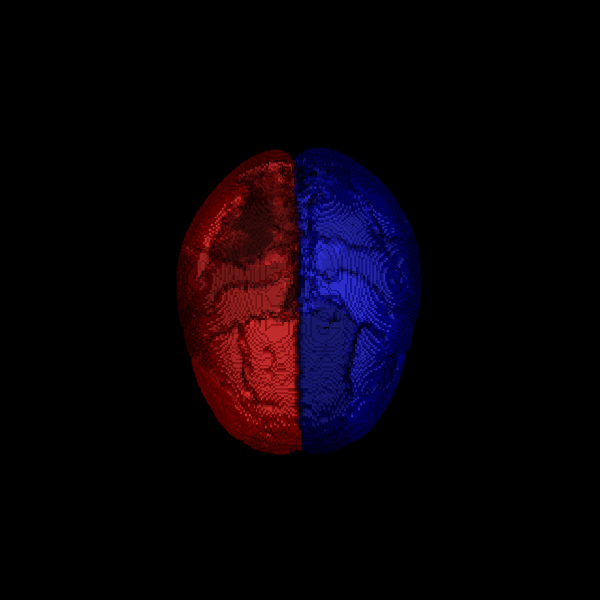
\includegraphics[width=1\textwidth]{desikan.png}
%\caption{Comparison of MSE between $\bar{A}$ (solid line) and $\hat{P}$ (dashed line) for desikan dataset while embedding the graphs into different dimensions with different size $M$ of the subsamples. The dimension chosen by the 3rd elbow of Zhu and Ghodsi is denoted in triangle, and chosen by USVT with threshold equals 0.7 is denoted in square.  Vertical intervals represent the 95\% confidence interval.  When $M$ is small, $\hat{P}$ outperforms $\bar{A}$ with a flexible range of the embedding dimension including what Zhu and Ghodsi selects.}
%\label{fig:desikan}
%\end{figure}
%
%\begin{figure}[!htb]
%\centering
%\includegraphics[width=1\textwidth]{CPAC200.png}
%\caption{Comparison of MSE between $\bar{A}$ (solid line) and $\hat{P}$ (dashed line) for CPAC200 dataset while embedding the graphs into different dimensions with different size $M$ of the subsamples. The dimension chosen by the 3rd elbow of Zhu and Ghodsi is denoted in triangle, and chosen by USVT with threshold equals 0.7 is denoted in square.  Vertical intervals represent the 95\% confidence interval.  When $M$ is small, $\hat{P}$ outperforms $\bar{A}$ with a flexible range of the embedding dimension including what Zhu and Ghodsi selects.}
%\label{fig:CPAC200}
%\end{figure}
%
%\begin{figure}
%\centering
%\begin{subfigure}{.33\textwidth}
%  \centering
%  \includegraphics[width=1.2\linewidth]{P_JHU.png}
%\end{subfigure}%
%\begin{subfigure}{.33\textwidth}
%  \centering
%  \includegraphics[width=1.2\linewidth]{Abar_JHU_m5.png}
%\end{subfigure}
%\begin{subfigure}{.33\textwidth}
%  \centering
%  \includegraphics[width=1.2\linewidth]{Phat_JHU_m5.png}
%\end{subfigure}
%\caption{Comparison between the mean of 454 graphs $P$ and two estimates $\bar{A}$ and $\hat{P}$ derived from a sample of size $M=5$ from JHU dataset while embedding the graphs into dimension $d=15$ selected by the 3rd elbow of ZG method.}
%\label{fig:adj_JHU_m5}
%\end{figure}
%
%\begin{figure}[!htb]
%\centering
%\includegraphics[width=1\textwidth]{Vertex_Diff_Phat_desikan.png}
%\caption{Top 5 regions of the brain (vertices in graphs) with largest absolute difference $|\hat{P} - P|$.}
%\label{fig:Vertex_Diff_Phat_desikan}
%\end{figure}
%
%\begin{figure}[!htb]
%\centering
%\includegraphics[width=1\textwidth]{Edge_Diff_Phat_desikan.png}
%\caption{Top 1\% (49) connections between regions (edges in graphs) with largest absolute difference $|\hat{P} - P|$.}
%\label{fig:Vertex_Diff_Phat_desikan}
%\end{figure}


\subsection{Simulation under the Full Rank Independent Edge Model}\label{sec:sim_iem}

While the theory we have developed is based on the assumption that the mean graph is low rank, as we have seen in Section~\ref{sec:corr_data}, $\hat{P}$ often performs well even when this assumption is false. 
To further illuminate this point, we perform a simulation under a full-rank independent edge model where we use the sample mean of the 454 graphs in the Desikan dataset as the probability matrix $P$.
As in the previous section, we simulated data sets of size $M=1,5$, and $10$ and used $\bar{A}$ and $\hat{P}$, where for $\hat{P}$ we varied the rank from 1 to 70.

Fig~\ref{fig:sim_desikan} shows resulting estimated MSE for $\bar{A}$ (solid line) and $\hat{P}$ (dashed line) for simulated data based on the full rank probability matrix $P$ shown in the left panel of Fig~\ref{fig:Matrix_desikan_m5}.
% Vertical lines at each dimension indicate the 95\% confidence intervals for the MSE.
We see that the results are very similar to those presented in section~\ref{sec:corr_data}.
When $M$ is small, $\hat{P}$ outperforms $\bar{A}$ with a flexible range of the embedding dimension including those selected by the Zhu and Ghodsi method while when $M$ is large enough, both estimators perform very well.
So $\hat{P}$ does a good job even when the low rank assumption of the model is violated. This simulation again shows the robustness of $\hat{P}$ to deviations from the RDPG model.


\begin{figure}[!htb]
\centering
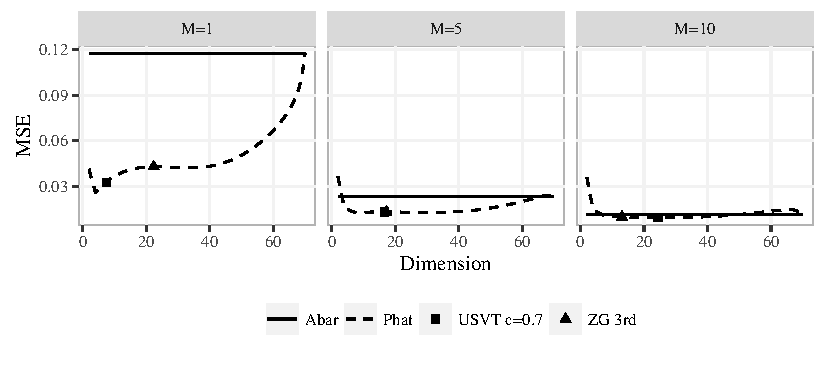
\includegraphics[width=1\textwidth]{sim_desikan.pdf}
\caption{Comparison of MSE between $\bar{A}$ (solid line) and $\hat{P}$ (dashed line) for simulated data with different sample sizes $M$ based on the sample mean for the Desikan dataset. Again, the average of dimensions selected by the USVT method (square) and the ZG method (triangle) tend to nearly approximate the optimal dimension. 
Overall, we that the structure of these plots well approximates the structure for the real data indicating that performance for the independent edge model will tend to translate in structure to non-independent edge scenarios.}
\label{fig:sim_desikan}
\end{figure}



\section{Discussion}

% In this paper, we propose using low-rank methods to estimate the mean of a collection of graphs.
Motivated by the RDPG model, our methodology takes advantage of the low-rank structure of the graphs by applying low-rank approximation to the entry-wise MLE. 
We give a closed form for the asymptotic relative efficiency between the entry-wise MLE $\bar{A}$ and our estimator $\hat{P}$ in the case of a stochastic blockmodel, demonstrating that when $N$ is sufficiently low-rank methods provide a substantial improvement.
Moreover, our estimator outperforms the entry-wise MLE in a cross validation analysis of the CoRR brain graphs and in low- and full-rank simulation settings.
These results illustrate that $\hat{P}$ performs well even when the low-rank assumption is violated and that $\hat{P}$ is robust and can be applied in practice.

One of the key observations from our real data analysis was that the largest improvements using the low-rank method occurred when the number of graphs $M$ was small and that it provided only minor improvements when $M$ is large. 
However, even in large scale studies the low-rank methods will be useful for estimating graph means for subpopulations, for example the population of females over 60 with some college education.
In another direction, \citet{durante2014nonparametric} used low-rank deviations from a full rank population mean to model collections of graphs and our methods could be easily adapted to these ideas.


% \subsection{Future Work}
% In this paper, we assume that the adjacency matrix is observed without contamination.
% However, generally there will be noise in practice and accounting for this noise with other more robust methods . With contaminations, robust estimators like ML$q$E is preferred. If an estimator can not only inherit robustness from the robust estimators but also has small variance by taking advantage of the low rank structure of the graphs, it will be very useful.

% Meanwhile, estimating the rank of the graph structure accurately will certainly help improve the performance of the estimator $\hat{P}$. Now we are using Zhu and Ghodsi's method and USVT, but there is still a lot of space for improvement, especially in this particular case.

While the low-rank methods considered in this paper will often offer substantial improvements, further refinements of these methods are still necessary.
For example, we assume that the adjacency matrix is observed without contamination, however, in practice there will be noise in the observed graph and accounting for this noise with other more robust methods is necessary.
This may be especially fruitful when each graph has weighted edges and the weights themselves have noisy or heavy-tailed distributions.
Rank-based methods and robust likelihood methods could be very useful in that case. 

 % With contaminations, robust estimators like ML$q$E is preferred. If an estimator can not only inherit robustness from the robust estimators but also has small variance by taking advantage of the low rank structure of the graphs, it will be very useful.

Another issue that arose in our analysis of the connectome data set was the presence of structural ones in the mean graph for the population. 
These structural ones appear since edges between certain regions of the brain are present in all or nearly all members of the healthy population. 
The low-rank methods tend to miss these always present edges while the sample mean will always capture them.
Detecting and incorporating structural ones and zeros could yield methods that share the best elements of both methods considered here.

For the CoRR data set, we used a cross validation framework where we compared the estimates based on a subsample to the mean for the held-out set. 
Another option would be to compare the estimates $\bar{A}$ and $\hat{P}$ to the mean for the entire population including the subsample.
Both of these analyses lead to very similar results in the cases presented above but for various reasons one may prefer one analysis over another.
The cross validation method is most reasonable from a prediction perspective where prediction about new samples is of interest.
If instead, one is interested in learning directly about the mean of a population, especially a finite population, the sub-sampling approach may be the most logical choice.

\section{Methods}

\subsection{Choosing Dimension}
\label{section:dim_select}
Often in dimensionality reduction techniques, the choice for dimension $d$, relies on analyzing the set of the ordered eigenvalues, looking for a ``gap'' or ``elbow'' in the scree-plot. \citet{zhu2006automatic} present an automated method for finding this gap in the scree-plot that takes only the ordered eigenvalues as an input and uses Gaussian mixture modeling to find these gaps.
The mixture modeling results in multiple candidate dimensions or elbows and our analysis indicated that underestimating the dimension is much more harmful than overestimating the dimension.
For this reason, we use the 3rd elbow in the experiments performed in this work.

Universal Singular Value Thresholding (USVT) is a simple estimation procedure proposed by \citet{chatterjee2015matrix} that can work for any matrix that has ``a little bit of structure''. 
In our setting, it selects the dimension $d$ as the number singular values that are greater than a constant $c$ times $\sqrt{N/M}$.
The specific constant $c$ must be selected carefully based on the mean and variance of the entries and since again we found that overestimating the dimension was not overly harmful, we chose a relatively small value of $c=0.7$.

Overall, selecting the appropriate dimension is a challenging task and numerous methods could be applied successfully depending on the setting.
On the other hand, we have observed that in our setting many dimensions will yield nearly optimal mean square errors and so efforts to ensure the selected dimension are in the appropriate range are more important than finding the singular best dimension.



\subsection{Graph Diagonal Augmentation}
\label{section:diag_aug}
The graphs examined in this work have no self-loops and thus the diagonal entries of the adjacency matrix and the mean graph are all zero.
However, when computing the low-rank approximation, these structural zeros lead to increased errors in the estimation of the mean graph. 
While this problem has been investigated in the single graph setting, with multiple graphs, the problem is exasperated since the variance of the others entries is lower, so the relative impact of the bias in the diagonal entries is higher.

\citet{marchette2011vertex}  proposed the simple method of imputing the diagonals to be equal to the average of the non-diagonal entries for the corresponding row.
Earlier, \citet{scheinerman2010modeling} proposed using an iterative method to impute the diagonal entries.
In this work we combine these two ideas by first using the row-average method  (see Step 3 of Algorithm~\ref{algo:basic}) and then using one step of the iterative method (see Step 6 of Algorithm~\ref{algo:basic}).
Note that when computing errors, we omit the diagonal entries since these are known to be zero.



\subsection{Dataset Description}
\label{section:data}
The original dataset is from the Emotion and Creativity One Year Retest Dataset provided by Qiu, Zhang and Wei from Southwest University available at the Consortium for Reliability and Reproducibility (CoRR) \cite{zuo2014open, gorgolewski2015high}. It is comprised of 235 subjects, all of whom were college students. Each subject underwent two sessions of anatomical, resting state DTI scans, spaced one year apart. Due to incomplete data, only 454 are available.

When deriving MR connectomes, the NeuroData team parcellates the brain into groups of voxels as defined by anatomical atlases \cite{neurodata, kiar2016graph}. The atlases are defined either physiologically by neuroanatomists (Desikan and JHU), or are generated using an automated segmentation algorithm (CPAC200).
% The graphs we are using are processed by NeuroData team from DTI data of the original dataset generated with different atlases (Desikan, JHU and CPAC200), each containing different region/node definitions. 
Once the voxels in the original image space are grouped into regions, an edge is placed between two regions when there is at least one white-matter tract, derived using a tractography algorithm, connecting the corresponding two parts of the brain.
The resulting graphs are undirected, unweighted and have no self-loops.


\subsection{Outline for the Proof of the Theorems}
\label{section:outline_proof}
Here we provide an outline of the proof Lemma~\ref{lm:VarPhat} which provides the approximate MSE of $\hat{P}$ in the stochastic blockmodel case.
The result depends on using the asymptotic results for the distribution of eigenvectors from \citet{athreya2013limit} which extend to the multiple graph setting in a straightforward way.

The first key observation, is that since $\bar{A}$ is computed from iid observations each with expectation $P$, $\bar{A}$ is unbiased for $P$ and $\mathrm{Var}(A_{ij}) = \frac{1}{M}P_{ij}(1-P_{ij}$.
The results of \citet{athreya2013limit} provide a central limit theorem for estimates of the latent position in a RDPG model for a single graph.
Since the variance of each entry is scaled by $1/M$ in $\bar{A}$, the analogous result for $\bar{A}$ is that the estimated latent positions will follow an approximately normal distribution with variance scaled by $1/M$ compared to the variance for a single graph. 
    
% When comparing two estimators, the first thing we need to consider is consistency.
% It is easy to see that $\bar{A}$ is unbiased as an estimate of $P$. 
% Moreover, since two latent positions are conditionally asymptotically independent by extended version of Theorem 1 in \citet{athreya2013limit}, we know $\hat{P}$ is consistent, as well as $\bar{A}$.

% Thus the relative efficiency between $\hat{P}$ and $\bar{A}$, which is equivalent to the ratio of mean square errors in this case, is a good indicate in comparison.

Since $\hat{P}_{ij} = \hat{X}_i^T \hat{X}_j$ is a noisy version of the dot product of $\nu_s^T \nu_t$ from section~\ref{section:sbm_rdpg} and each $\hat{X}_i$ are approximately independent and normal, we can use common results for the variance of the inner product of two independent multivariate normals \citet{brown1977means}.
After simplifications that occur in the stochastic blockmodel setting we can derive that the variance of $\hat{P}_{ij}$ converges to $\left( 1/\rho_{\tau_i} + 1/\rho_{\tau_j} \right) P_{ij} (1-P_{ij})/(N \cdot M)$ as $N \rightarrow \infty$. 
Since the variance of $\bar{A}_{ij}$ is $P_{ij} (1-P_{ij})/M$, the relative efficiency between $\hat{P}_{ij}$ and $\bar{A}_{ij}$ is approximately $(\rho_{\tau_i}^{-1} + \rho_{\tau_j}^{-1})/N$ when $N$ is sufficiently large.
    
The full proof is provided at https://www.overleaf.com/2776898cydwhv. 

\bibliography{Bib}
% \bibliographystyle{plain}


\end{document}